\subsection{Перебор состояний}

Код реализации среды исполнения и код реализации перебора должны быть отделены друг от друга ради того, чтобы иметь возможность писать сколь угодно сложные алгоритмы в checker-е.

\subsubsection{Модель акторов}

Для того, чтобы отделить алгоритм перебора исполнений от среды исполнения для отдельных узлов, будем рассматривать все узлы, на которых подразумевается  исполнение пользовательского кода (как клиентов, так и серверов), в модели акторов \cite{actor}. 

В этой модели все исполняемые сущности (в нашем случае – клиенты и серверы) представляются в виде однопоточных автоматов, которые объединены общей шиной сообщений. Схема взаимодействия внешнего мира с актором такова: актор реагирует на сообщение, адресованное ему, сменой своего состояния и посылкой новых сообщений во внешний мир.

Актор в model checker-е представлен в виде интерфейса IActor с методом HandleMessage (рис.~\ref{fig:actor}): этот метод вызывается model checker-ом. За реализацией этого интерфейса находится узел с пользовательским кодом, RPC и concurrency.

\begin{figure}[h]
    \centering
    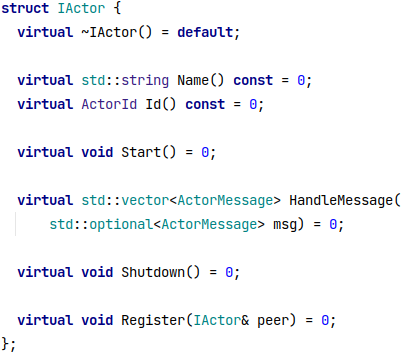
\includegraphics[width=0.75\textwidth]{img/actor.png}
    \caption{Интерфейс актора}
    \label{fig:actor}
\end{figure}

Строго говоря, код пользователя, исполняемый внутри узла, является недетерминированным, и считать узел детерминированным автоматом неверно. Но для model checker-а мы организуем псевдоконкурентное исполнение, оставляя за рамками проверку ошибок многопоточного кода, так как тестирование concurrency является отдельной задачей, для которой применяются те же техники, но в другом масштабе (fault-injection, thread sanitizer).

Стоит представлять себе систему в виде нескольких узлов, которые взаимодействуют через абстракцию физического уровня – сеть. Сеть является глобальным буфером, куда серверы-акторы складывают новые сообщения.

Таким образом, проверка всех достижимых в тесте состояний системы состоит в переборе всех возможных порядков доставки отправляемых узлами-акторами сообщений или, в терминах model checking, в переборе всех возможных ветвей в графе конфигураций.

\subsubsection{Схема перебора}

Model checker может использовать два способа обхода графа конфигураций: поиск в ширину и поиск в глубину. Обход поиском в ширину позволяет находить минимальное по количеству шагов исполнение, нарушающее инвариант \cite{demi}. Минус этого подхода состоит в том, что для него нужно иметь явное представление вершин графа, ведь если сохранять состояние в виде последовательности доставок сообщений, то на очередной итерации BFS приходится снова исполнять доставки в префиксе истории. Обход поиском в глубину позволяет неявно хранить состояние системы: стартуя из начального состояния системы идти по пути, переходя по ребрам за счет доставки сообщений. Мы выбираем обход поиском в глубину, так как из-за ограничения по ресурсам памяти не можем явно хранить состояние сложной распределенной системы.

Деталью перебора является следующее: в начале исполнения очередной ветви мы хотим инициализировать состояние системы, а в конце сбросить текущее состояние. 

В начале перебора ветви выполняется инициализация акторов. В буфер сети на данном этапе приходят все начальные сообщения. Далее происходит перебор, который по описанному алгоритму выбирает очередной индекс сообщения для доставки, извлекает из сети нужное сообщение и доставляет его, тем самым изменяя состояние актора-адресата. После этого буфер, возможно, пополняется новыми сообщениями. На последующих итерациях весь этот процесс повторяется.

\subsubsection{Ограничения}

При тестировании кода нас чаще всего интересует валидация модели согласованности. Такая гарантия является Safety свойством, потому что она представима в виде инварианта через накопление состояния об истории исполнения. Мы сфокусируемся на валидации только такого вида свойств.

Само тестирование будет подразумевать проверку инвариантов кода и не будет работать над проверкой устойчивости кода к перезагрузке узлов, сбоям диска, дрейфу часов и разрывам соединений. Для тестирования подобных сбоев в фреймворке существует режим детерминированной симуляции.

Сбои, состоящие в отказе узла, нет необходимости моделировать отдельно, так как отказ узла – это исполнение, где данный узел не изменяет своё состояние, и ему не доставляются сообщения.
